\begin{frame}{Problem}
  %\textcolor{tugreen}{\Large Problem:}
  \begin{itemize}
    \item How effectively can we classify bird species by analysing sound files using a convolutional neural network (CNN)?
  \end{itemize}
  \vspace{2mm}
  \textcolor{tugreen}{\Large Motivation:}
  \vspace{1mm}
  \begin{itemize}
    \item Classifying and observing different species of birds is of great interest for wildlife research
    \item But often you don't see the birds themselves and only hear their calls
    \item Differentiating bird species from sound recordings requires expert knowledge and is very time consuming
    \begin{columns}
      \column{.45\textwidth}
      \vspace*{-3mm}
      \begin{itemize}
        \item A CNN could be used to automatically identify different species by patterns in spectrograms of audio recordings
      \end{itemize}

      \column{.55\textwidth}
      \vspace{-2mm}
      \begin{figure}
        \centering
        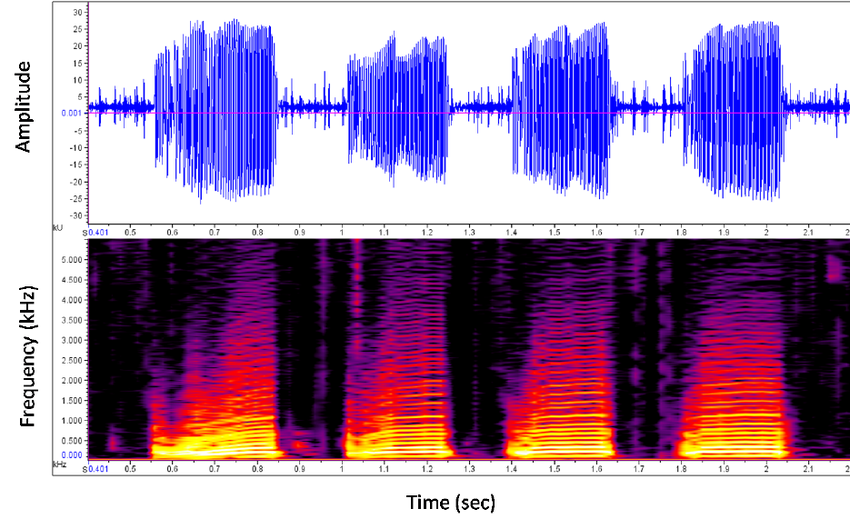
\includegraphics[width = .6\textwidth]{content/graphics/spectrogram.png}
        \caption*{\scriptsize \fullcite{Kat2009}}
      \end{figure}
    \end{columns}
  \end{itemize}
\end{frame}

\begin{frame}{Dataset}
  \only<1>{
  \vspace*{-16mm}
  \begin{itemize}
    \item Source: \href{https://www.kaggle.com/datasets/monogenea/birdsongs-from-europe}{\textcolor{blue}{www.kaggle.com/datasets/monogenea/birdsongs-from-europe}}
    \item Dataset contains sound recordings of 50 european bird species
    \begin{itemize}
      \item For each species there are $\num{43}$ .mp3 files of different length
      \item The recordings contain background noises etc. 
    \end{itemize}
    \item Additionally, a .csv file with metadata for all recordings is provided
    \begin{itemize}
      \item Species, location, recordist, date ...
    \end{itemize}
  \end{itemize}
  }
  \begin{figure}
    \centering 
    \includegraphics<2>[width=\textwidth]{content/graphics/dataframe.png}
  \end{figure}
  \only<3>{
    \vspace*{-16mm}
    \begin{itemize}
      \item Source: \href{https://www.kaggle.com/datasets/monogenea/birdsongs-from-europe}{\textcolor{blue}{www.kaggle.com/datasets/monogenea/birdsongs-from-europe}}
      \item Dataset contains sound recordings of 50 european bird species
      \begin{itemize}
        \item For each species there are $\num{43}$ .mp3 files of different length
        \item The recordings contain background noises etc. 
      \end{itemize}
      \item Additionally, a .csv file with metadata for all recordings is provided
      \begin{itemize}
        \item Species, location, recordist, date ...
      \end{itemize}
      \item Original data from \href{https://xeno-canto.org/}{\textcolor{blue}{xeno-canto.org/}}
      \begin{itemize}
        \item A website for sharing and classifying wildlife sound recordings
      \end{itemize}
      \item Each audio file is licensed individually by its author
      \begin{itemize}
        \item The individual licenses are listed in the .csv 
        \item Usually they are licensed as \textit{Creative Commons}
      \end{itemize}
    \end{itemize}
  }
\end{frame}

\begin{frame}{Comparison with alternative method}
  \begin{itemize}
    \item Using a CNN is the most obvious and most promising approach for such a problem 
    \item An alternative method could e.g. make use of a \textit{KNN} classifier
  \end{itemize}
  \vspace{2mm}
  \textcolor{tugreen}{\large Strategy:}
  \begin{enumerate}
    \item Extract meaningful features from the audio files 
    \begin{itemize}
      \item Zero crossing rate, RMS energy (loudness), energy
      \item Spectral analysis using \textit{FFT} or \textit{Lomb-Scargle}
      \item Most prominent frequencies, spectral centroid/flux/spread etc.
    \end{itemize}
    \item Train k-nearest neighbours algorithm 
    \item Compare performance
  \end{enumerate}
  \vspace{2mm}
  \textcolor{tugreen}{\large Performance measure:}
  \begin{itemize}
    \item Accuracy / F1-score
  \end{itemize}
\end{frame}
